% it/figures/sdg/sdg_alignment.tex — versione italiana
\begin{figure}[!ht]
    \centering
    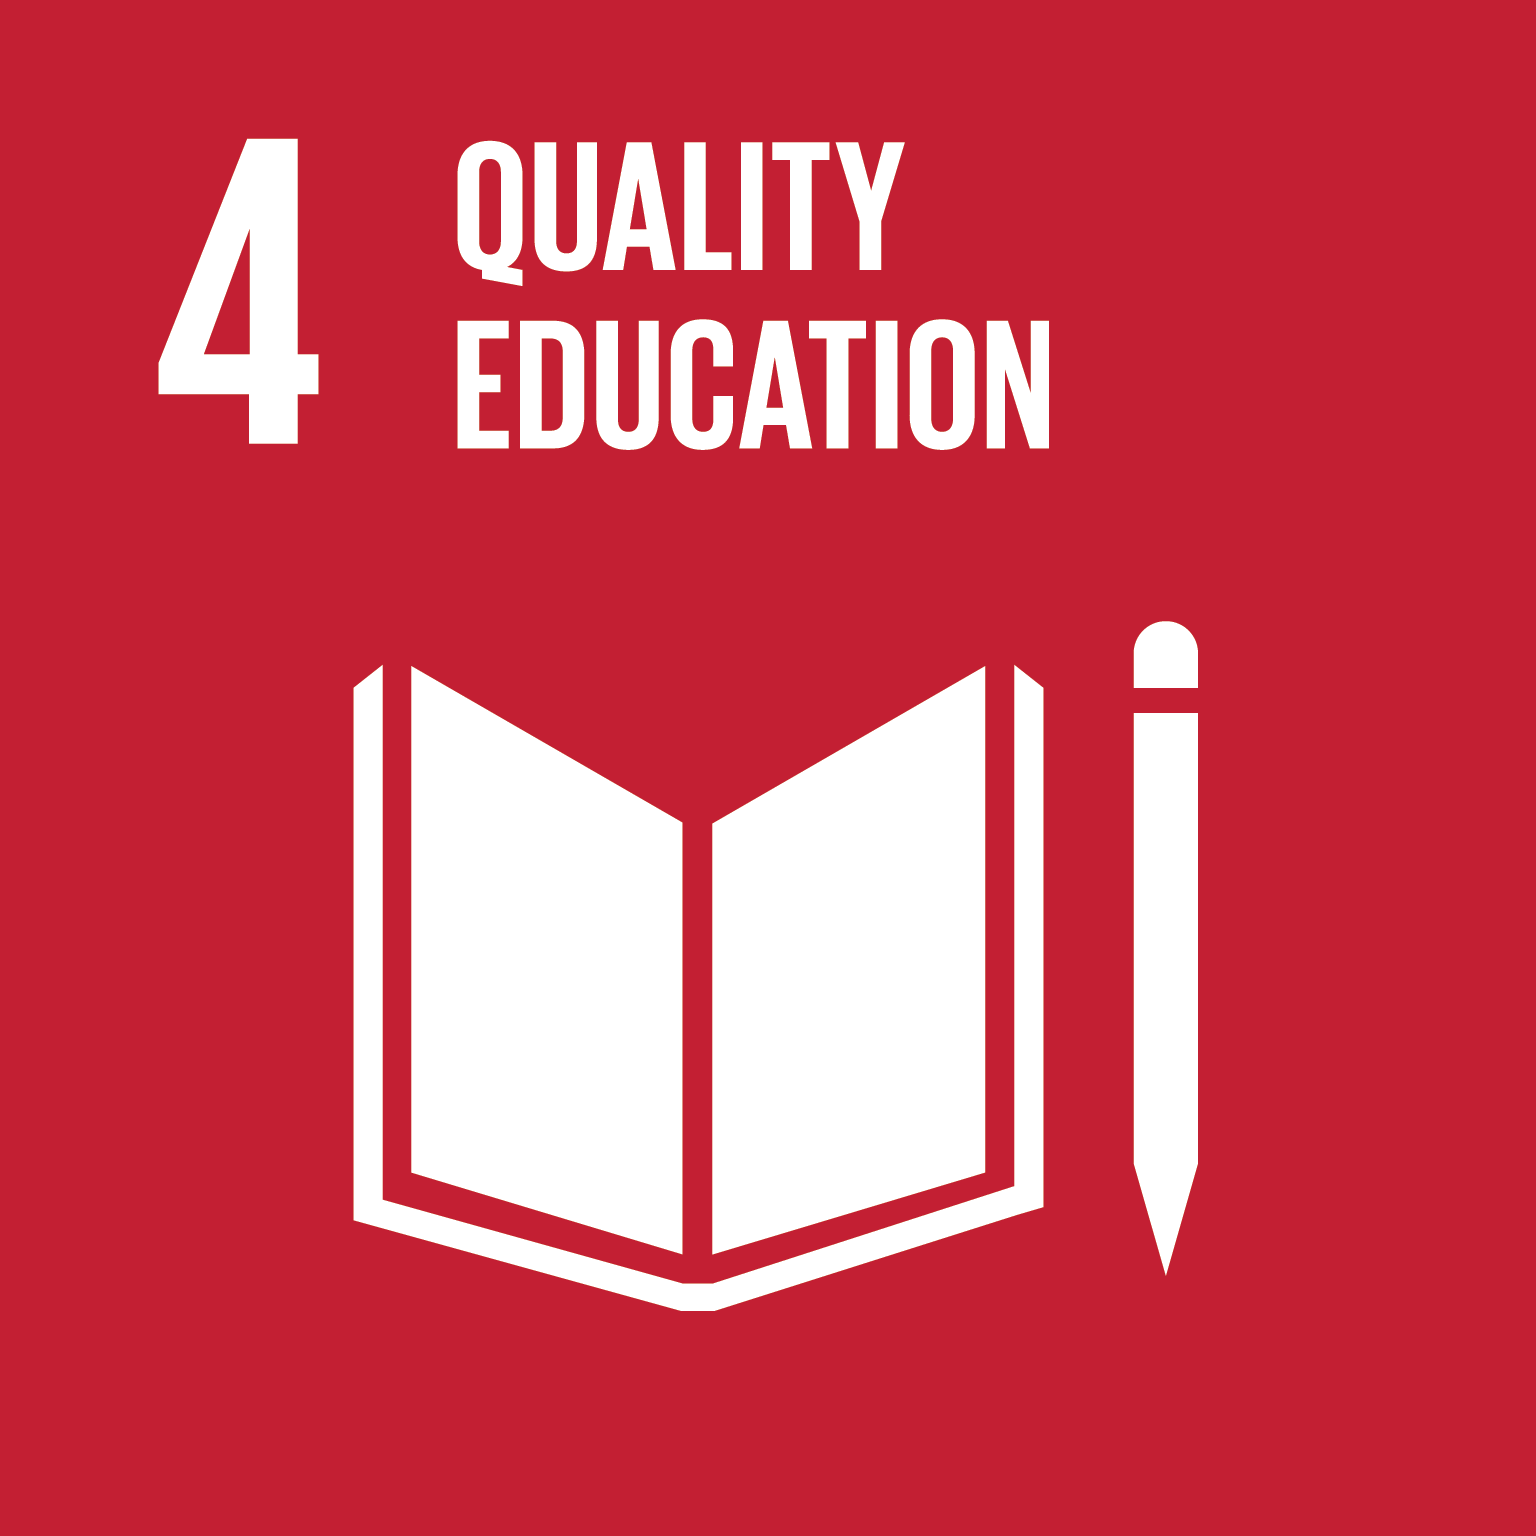
\includegraphics[height=4cm]{figures/sdg/sdg4.png}\hfill
    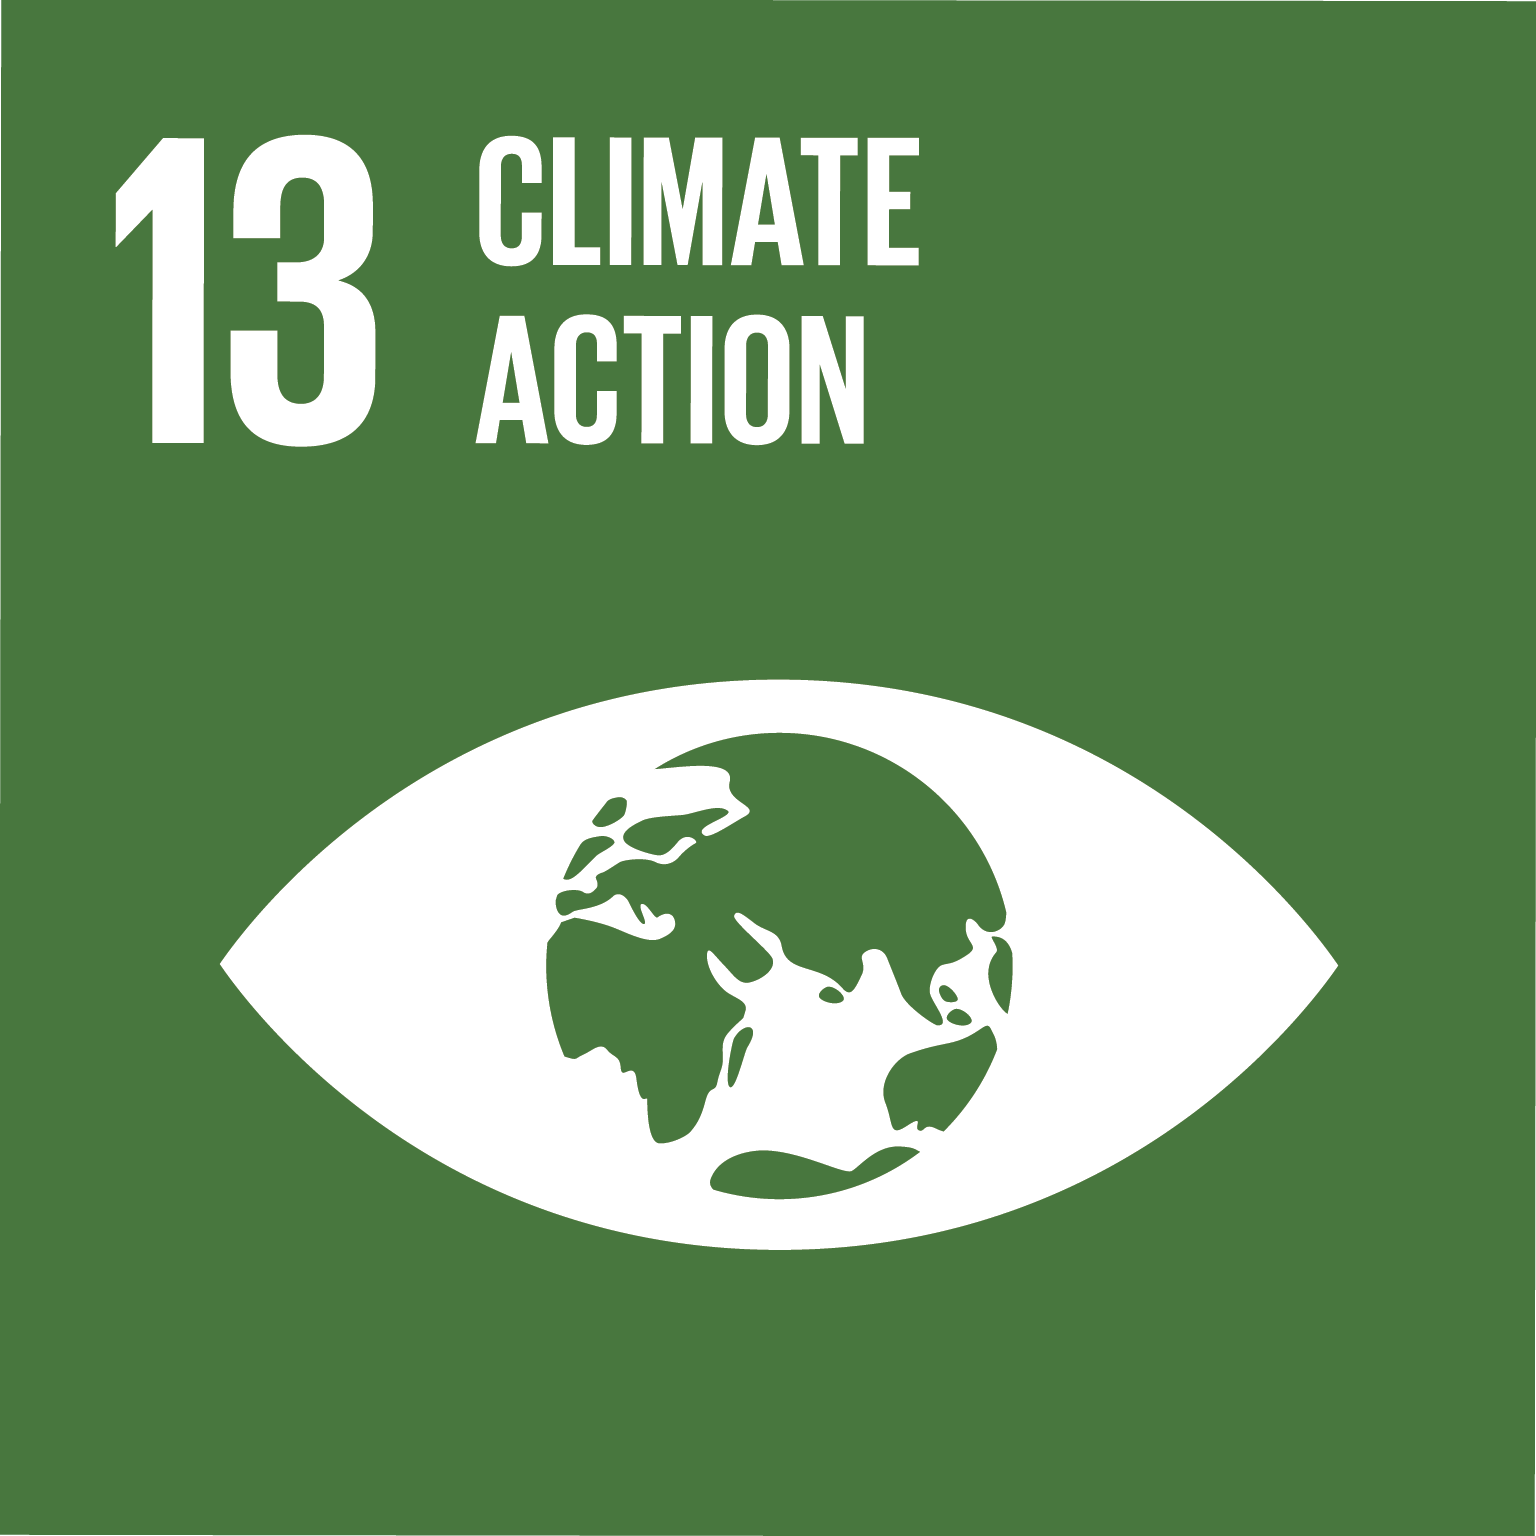
\includegraphics[height=4cm]{figures/sdg/sdg13.png}\hfill
    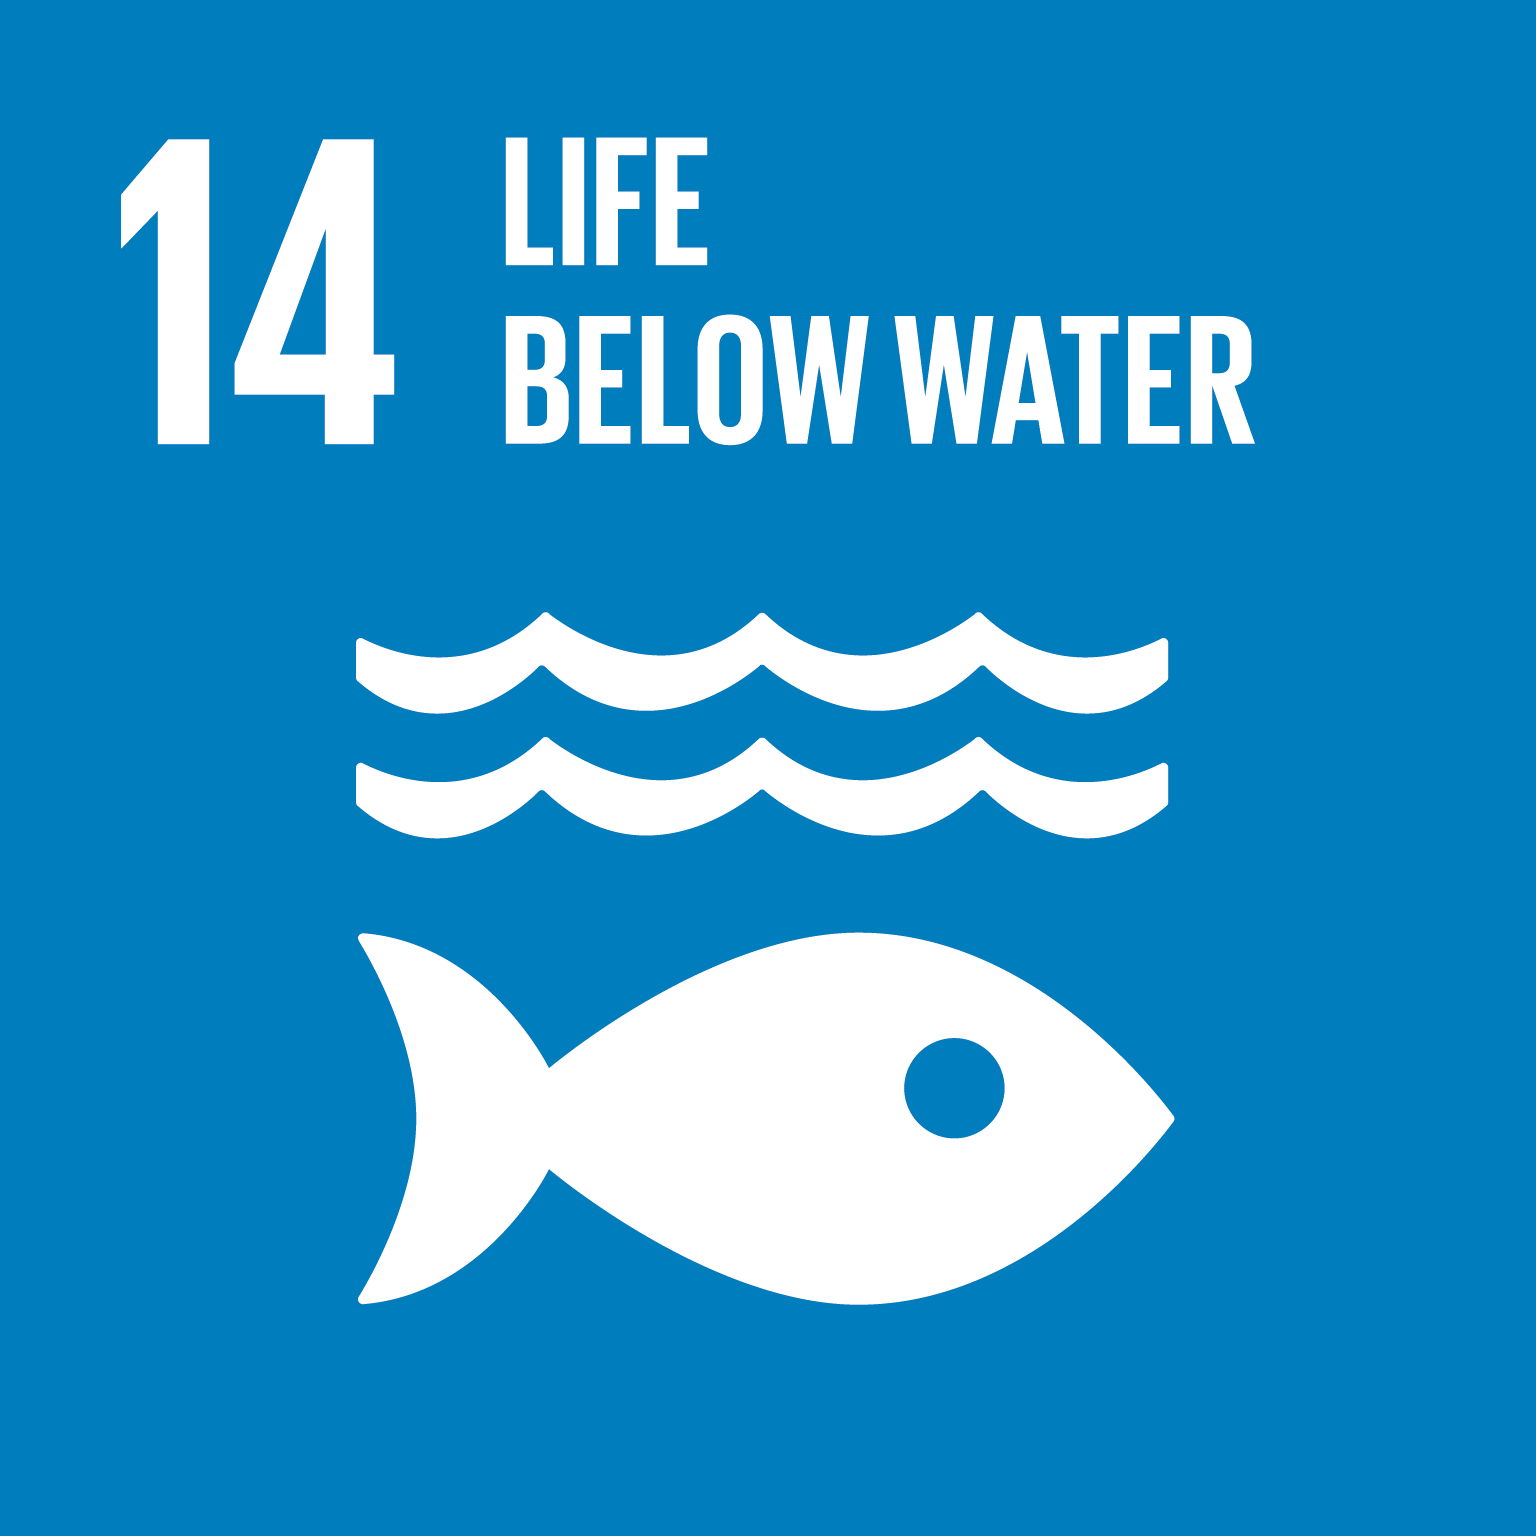
\includegraphics[height=4cm]{figures/sdg/sdg14.png}
    \caption[Obiettivi di Sviluppo Sostenibile affrontati da questa tesi.]{\textbf{I
    tre Obiettivi di Sviluppo Sostenibile a cui questa tesi contribuisce.} SDG~13
    (Lotta al cambiamento climatico), in particolare il target~13.3 su educazione,
    consapevolezza e capacità; SDG~4 (Istruzione di qualità), sul rendere accessibile
    la conoscenza complessa; e SDG~14 (La vita sott'acqua), poiché l'AMOC fa parte del
    sistema oceanico. Icone \textcopyright~Nazioni Unite. Il contenuto di questa
    pubblicazione non è stato approvato dalle Nazioni Unite e non ne riflette le
    opinioni.}
    \label{fig:sdg-alignment}
\end{figure}
